\documentclass[14pt]{article}
\usepackage[letterpaper,top=3.5cm,bottom=3.5cm,left=2cm,right=2cm]{geometry}
\usepackage{import}
\usepackage{amsmath}
\usepackage{graphicx}
\usepackage[svgnames]{xcolor}
\usepackage[colorlinks=true, allcolors=blue]{hyperref}
\usepackage{listings}
\usepackage{minted}
\usepackage{url}
\usepackage[backend=bibtex, sorting=none]{biblatex}
\usepackage{subfiles} % Best loaded last in the preamble
\graphicspath{ {images/} }
\addbibresource[]{bibliography.bib}

\title{
        Autonomous and Intelligent Systems \\
        Internship report
}
\author{Jos\`e Dalla Torre \\ 143216@spes.uniud.it}
\date{April 2026}

\begin{document}
\maketitle
\newpage
\tableofcontents
\newpage
\section{Evaluating LoRa Comunication Protocol}
\newpage
\section{Setup}
In this section is presented how to setup correctly the OS for the RaspberryPi, the repository and the libraries used by the proposed solution. \\
After setting up the Raspberry Pi following the \href{https://www.raspberrypi.com/documentation/computers/getting-started.html}{official guide} it's necessary to enable SPI (Serial Peripheral Interface) selecting "Interface" and then "SPI" after using the following command.
\begin{minted}{bash}
sudo raspi-config
\end{minted}
Then it's necessary to download the WiringPi library used to access GPIO with high performance. To do so requires the following command:
\begin{minted}[breaklines]{bash}
wget https://github.com/WiringPi/WiringPi/releases/download/3.16/wiringpi_3.16_armhf.deb
sudo dpkg -i wiringpi_3.16_armhf.deb
\end{minted}
Lastly it's necessary to modify two files inside the LoRa-RaspberryPi folder:
\begin{itemize}
        \item Makefile: \#PYTHONVER=python3.11 needs to match system's Python version:
        \item lora.c: it's necessary to add \#define PY\_SSIZE\_T\_CLEAN on the first line for compatibility with new versions of Python.
\end{itemize}
To check out which version of Python it's installed use this command:
\begin{minted}{bash}
python3 --version
\end{minted}
These two changes are already been made in the \href{https://github.com/josedallatorre/SkyCLI/}{updated repository} with the proposed solution inside the "src" folder. \\ 
Finally it's necessary to compile with the following command:
\begin{minted}{bash}
make all
\end{minted}
\section{Proposed solution}
In this section is presented the proposed solution, starting with its folder structure then explaining the code for the sender and the receiver. Lastly the code for the analysis will be presented.
\subsection{Folder structure}
Inside the repository there are three folder:
\begin{itemize}
        \item report: this folder can be ignored since it has been used to store the files needed for this report.
        \item src: inside this folder there's the code for the receiver and the sender, then the libraries used by both. There's also a utils folder with helper functions for logging and converting digits.
        \item analysis: inside this folder there's a notebook with the code for the analysis that will be explained later.
\end{itemize}
\subsection{Sender}
Insider the sender folder there are two files: \\
hf-sender.py: this file was used to test the maximum message sending capacity. It wasn't used during the last tests, the reasons will explained later. \\
During the tests with hf-sender it has been observed that the messages were corrupted or the receiver didn't receive them correctly. \\
After reading this \href{https://www.thethingsnetwork.org/docs/lorawan/spreading-factors/}{article} the code has been updated in a new file called sender.py
In this new file the messages were delayed based on the airtime. \\
To calculate the airtime it has been used the formula defined in \href{https://www.mouser.com/pdfdocs/semtech-lora-modem-design.pdf}{Semtech's LoRa Modem Designer's Guide (AN1200.13)}. \href{https://avbentem.github.io/airtime-calculator/ttn/eu868}{This} website visually explain how airtime is influenced by factor like payload size and data rate. \\
To start sending messages use the following command inside the "src" folder:
\begin{minted}[breaklines]{bash}
python -m sender.sender 
\end{minted}
\subsection{Receiver}
Insider the receiver folder there are two files: \\
receiver.py: this file was used to test if the receiver could actually receive and log the message. After the first test it has been observed that looping through a fixed range of values isn't the best approach since the sender and the receiver can't synchronize. \\
After this consideration it has been decided to choose a fixed amount of time, in this case 2 minutes, to send and receive messages. \\
To start receiving messages use the following command inside the "src" folder:
\begin{minted}[breaklines]{bash}
python -m receiver.hf-receiver 
\end{minted}
\subsection{Utils}
Inside the utils folder there are two files:
\begin{itemize}
        \item conversion.py: contains two helper function that convert a positive number to its digit representation in base b.
        \item loggin.py: contains one helper function that create a logger and setup the folders to save the data from the communicator.
\end{itemize}
The first file has been created to solve the following problem: since the LoRaRaspberryPi library only transmit bytes of data it's necessary to convert the counter to a list of digits in base 255. \\
It's has been used a list of digits to be able to send a counter greater than 255.
\subsection{Analysis}
In this section will be presented the data analysis based on the tests made outside the SMACT 3 laboratory. \\
In total 7 test has been done:
\begin{itemize}
        \item  first test: communication in the parking lot of the laboratory, ~100 meters. LoRa spreading factor set to 7.
        \item  second test: same as the first but with a spreading factor set to 12.
        \item  third test: from the water storage outside the canteen to the trees, ~100 meters LoRa spreading factor set to 12.
        \item  fourth test: same as the first but between the RaspberryPis there were more trees.
        \item  fifth test: from the tree next to the canteen to "Canale Ledra". LoRa spreading factor set to 12.
        \item  sixth test: communication from Autonomous System laboratory to Cybersecurity laboratory. LoRa spreading factor set to 10
        \item  seventh test: communication inside the Autonomous System laboratory. LoRa spreading factor set to 10.
\end{itemize}
The analysis starts with the installation of the required packages and the definition of the function already presented before. \\
The collected data was preprocessed to remove inconsistencies. \\
This step revealed:
\begin{itemize}
        \item 5 errors in the sender logs
        \item 1 invalid message in the receiver logs
\end{itemize}
Given the small proportion of errors relative to the total number of transmitted messages, their impact on the overall results is minimal. Therefore, they are not expected to significantly affect the validity of the analysis. \\
The first part of the analysis evaluates the reliability of the communication by measuring the proportion of successfully received messages. \\
The results are summarized in \ref{fig:pie_chart_received_mgs}, which shows the distribution of message outcomes for each test. \\
Since the sender and receiver were manually synchronized, some messages were transmitted before the receiver was ready. These messages are not classified as transmission errors but are instead considered a separate category. \\
The results indicate that:
\begin{itemize}
        \item Communication reliability is generally high across all tests
        \item Only one invalid message was observed (Test 2)
        \item Sender-side logging errors occurred sporadically but did not affect reception significantly
\end{itemize}
\\
This suggests that the LoRa communication setup is robust under the tested conditions, even in the presence of obstacles and varying spreading factors. \\
\begin{figure}[h]
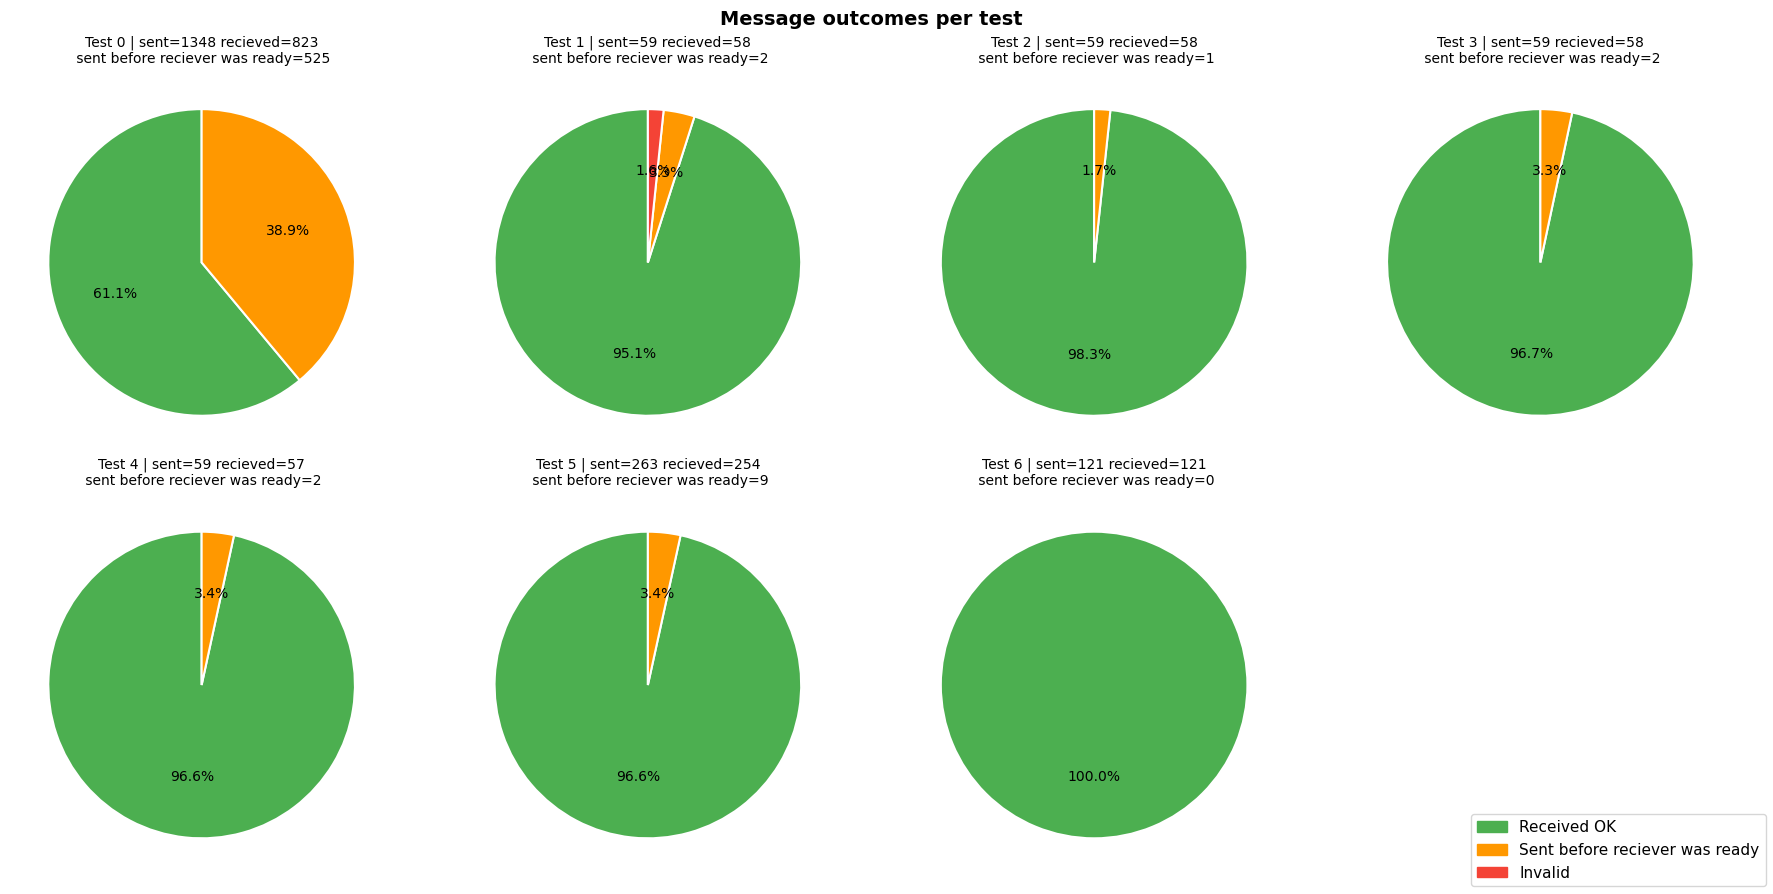
\includegraphics[width=\textwidth]{pie_chart_received_mgs}
\caption{Pie charts of the message outcomes per test}
\label{fig:pie_chart_received_mgs}
\centering
\end{figure}
The second part of the analysis focuses on communication latency.
In particular, the following metrics were considered:
\begin{itemize}
        \item Median latency (typical performance)
        \item Maximum latency (worst-case scenario)
        \item 99th percentile latency (tail behavior)
\end{itemize}
These metrics allow the identification of latency spikes and help define acceptable performance bounds.
The results are illustrated in:
\begin{itemize}
        \item \ref{fig:latency_per_test}: latency per message
        \item \ref{fig:latency_distribution}: latency distribution per test
        \item \ref{fig:latency_heatmap}: latency heatmap
\end{itemize}

The analysis shows that:

Higher spreading factors tend to increase latency due to longer airtime
Latency variability is more pronounced in outdoor environments with obstacles
Indoor tests exhibit more stable latency, likely due to controlled conditions

Overall, the observed latency values remain within acceptable limits for low-throughput IoT communication scenarios.



The analysis continues with checking on latencies. In particular the focus in on the median, maximum and 99-th percentile to highlight possible spikes and to define acceptable bounds.
\begin{figure}[h]
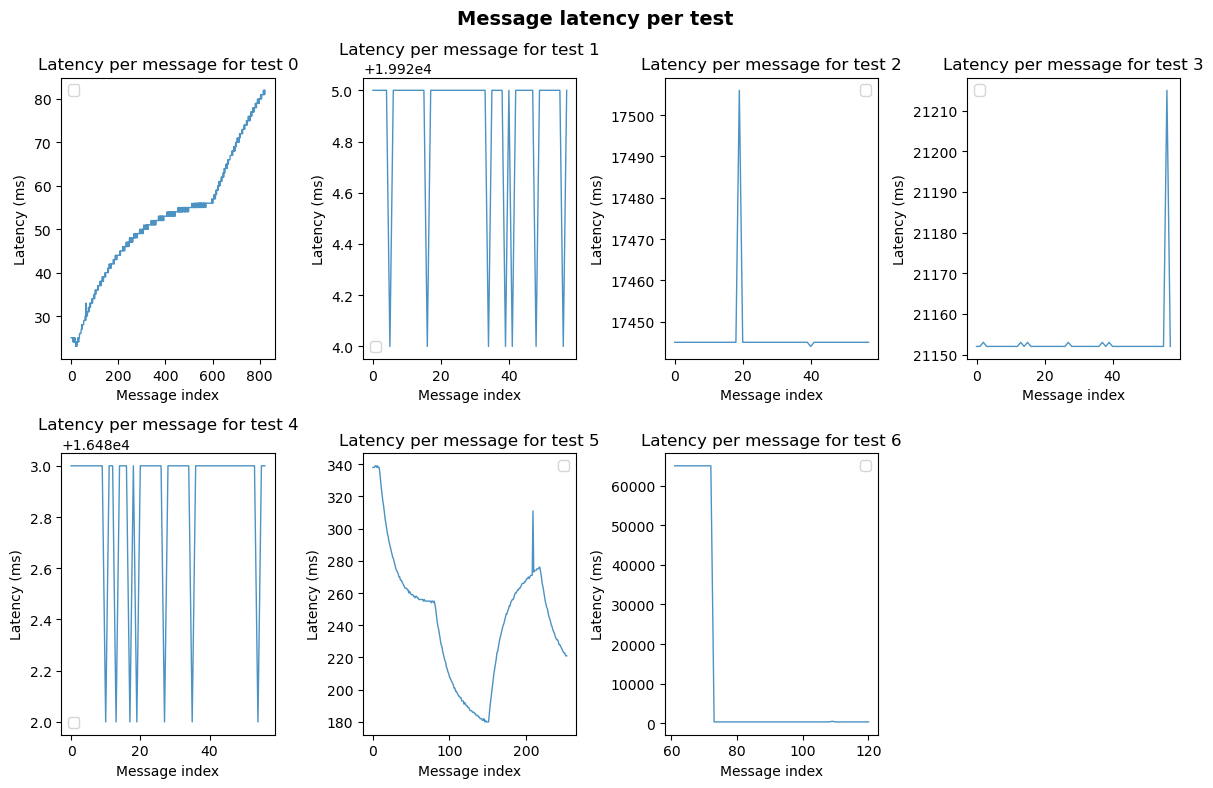
\includegraphics[width=\textwidth]{latency_per_test}
\caption{}
\label{fig:latency_per_test}
\centering
\end{figure}
\\
askjd
\begin{figure}[h]
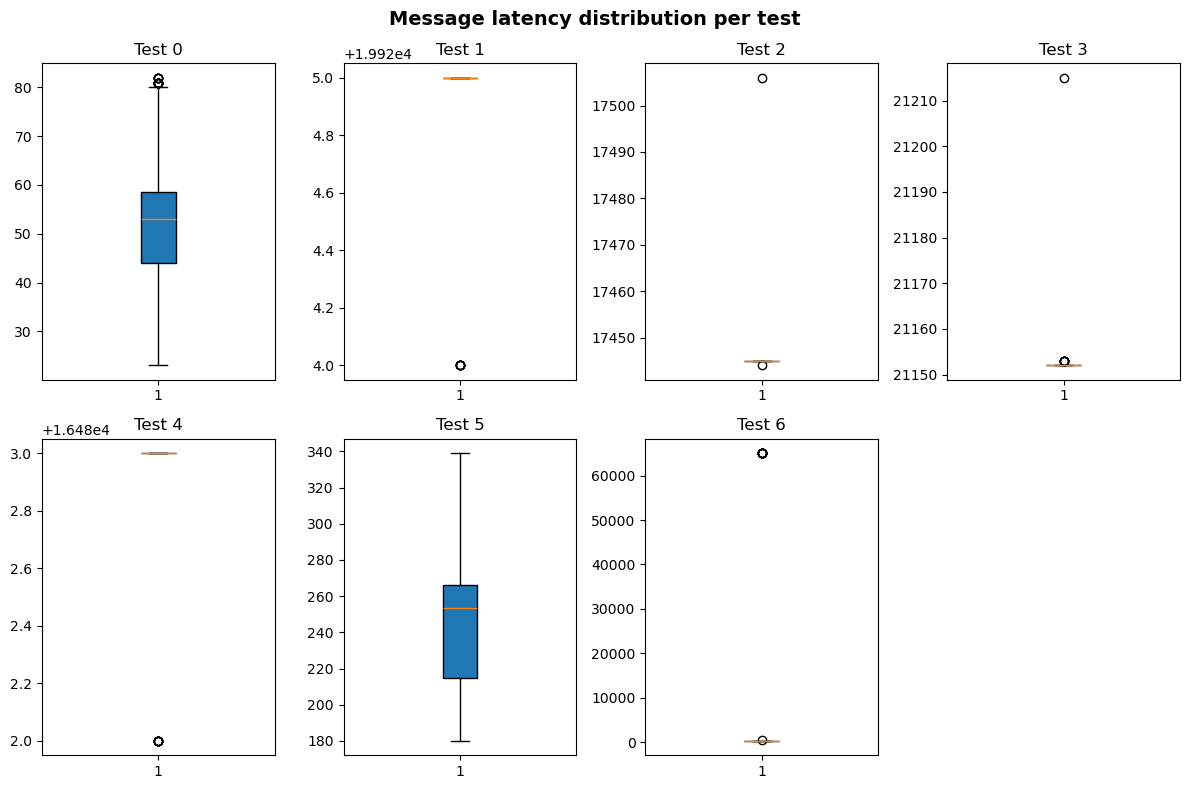
\includegraphics[width=\textwidth]{latency_distribution}
\caption{}
\label{fig:latency_distribution}
\centering
\end{figure}
\\
askjd
\begin{figure}[h]
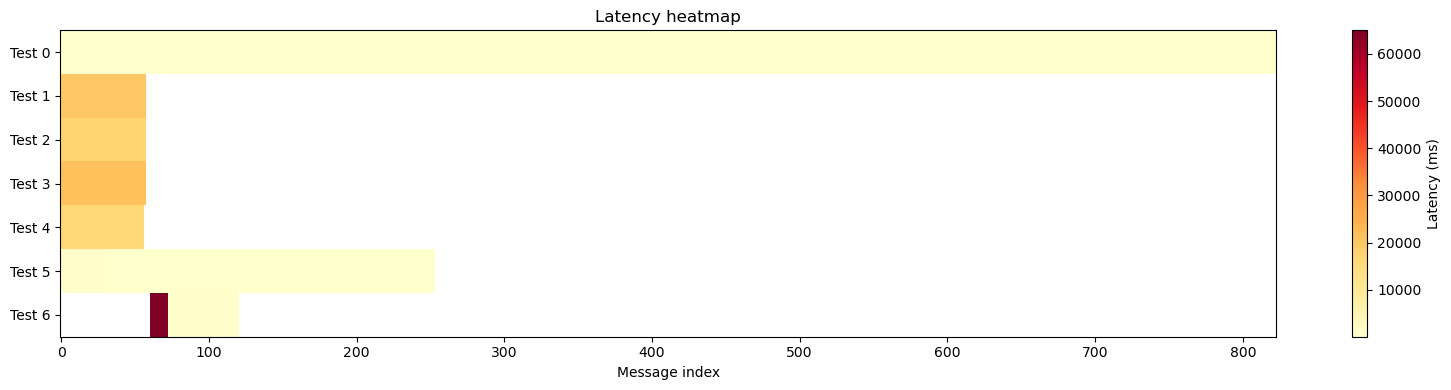
\includegraphics[width=\textwidth]{latency_heatmap}
\caption{Pie charts of the message outcomes per test}
\label{fig:latency_heatmap}
\centering
\end{figure}
\\
askjd
\newpage
\newpage
\section{Conclusion}
Conclusion
\appendix
\newpage

%\bibliographystyle{plainurl} 
\printbibliography

\end{document}